\section{はじめに}

本書は初めてSCALEモデルを利用するユーザー向けに、SCALE-LESモデルについて解説したユーザーズガイドです。
第\ref{sec:overview}章でSCALEの概要について説明します。第\ref{sec:install}章で必要な環境、
およびインストール方法を説明します。つづいて、第\ref{sec:tuto_ideal}章では理想実験、
第\ref{sec:tuto_real}章では現実大気実験の簡単な例を挙げて実行方法を説明します。
第\ref{sec:install}章から第\ref{sec:tuto_real}章まではひとつながりの
チュートリアルになっており、前章の経験や結果に基づいて説明する部分がありますので注意してください。
第\ref{sec:advance}章ではチュートリアルでは説明しなかった実行方法の詳細、
機能やツールについて説明します。

本書中の不明点やお気づきの点がございましたら、
SCALE user's メーリングリスト \verb|scale-user@riken.jp|までご連絡ください。



\subsection{SCALEの特徴}
SCALEは計算機を用いて気象・気候科学の問題にアプローチする際に、ユーザーが研究を進めやすいように
事前処理から数値モデル計算、解析に至るまですべての過程を網羅する計算ライブラリの開発を
目指したソフトウェアであり。SCALEは下記に挙げるような特徴を持つ。
\begin{itemize}
\item SCALEは、 ``Scalable Computing for Advanced Library and Environment''の略である.
\item SCALEは、フリーソフトウェアである。「BSD-2ライセンス」においてフリーソフトウェア
として提供されており、商用、非商用に関わらず自由な利用・改変が可能なソフトウェアである。
\item SCALEには、SCALE-LESモデル、SCALE-GMといった組み上げ済みの数値モデルが含まれている。
\item SCALEには、次節で説明する様々なコンポーネントが導入されており、必要に応じて取り替えることが可能性である。
\end{itemize}

ライセンスの詳細は、トップディレクトリ直下の``\verb|scale/LICENSE|''のファイルに記述されている。
SCALEの使用前に一読しておくこと。

\subsection{SCALE-LESモデルの構成}
現在,SCALE-LESモデルとして組み込まれているコンポーネントは下記のものである.
詳細なモデル構成や差分化手法については,\cite{scale_2015}や\cite{nishizawa_2015}を参照されたい.\\

\textcolor{red}{\bf 下記のリストは表に置き換えて、選択可能なものと、そうでないものが明確なようにまとめる}


\noindent{\bf フレームワーク関係}

\begin{itemize}
 \item Cartesian グリッドシステム(Arakawa C-grid)
 \item Cartesian ベースMPI通信
 \item Map-projection \& Map-factors
 \item Nesting システム(1-way, offline, and online)
 \item 複数事例一括実行 システム(Bulk Job システム)
 \item gtoolベースnetcdf4ファイル I/O
 \item WRF-ARW、NICAM、その他GrADSフォーマットでの初期値・境界値データ読み込み
\end{itemize}

{\bf 力学コア関係}

\begin{itemize}
 \item 方程式系: 3次元完全圧縮流体方程式
 \item 数値解法: HE-VE,  HE-VI,HI-VIスキームから選択可能
 \item 空間差分: 4次中央差分
 \item 時間差分: 3次ルンゲクッタスキーム
 \item 非負保証: FCTスキーム
 \item 数値フィルター: 4次Hyper diffusion
 \item 地形: Terrain-followingスキーム
\end{itemize}

{\bf 物理過程}

\begin{itemize}
 \item 乱流過程: Smagorinsky-Lilly typeのサブグリッドモデル (\cite{smagorinsky_1963}; \cite{lilly_1962}), 
MYNN2.5境界層モデル (\cite{my_1982},\cite{nakanishi_2004})から選択可能
 \item 雲微物理: Kessler type バルクモデル(Kessler 1969),6-class single moment バルクモデル(tomita 2006),
6-class double moment バルクモデル(\cite{sn_2014}),ビン法雲モデル(\cite{suzuki_etal_2010})から選択可能
 \item 放射過程: MSTRN (Sekiguchi and Nakajima 2008)
 \item 地表面モデル
  \begin{itemize}
   \item 陸面モデル: バケツモデル(バルク交換係数は \cite{beljaars_1991}; \cite{wilson_2001})
   \item 海洋モデル:(スラブモデル)
   \item 都市モデル: 単層キャノピーモデル(\cite{kusaka_2001})
  \end{itemize}
\end{itemize}

上記に加えて,SCALE-LESモデル本体のドライバー,現実事例の計算に必要な地形や土地利用データを作成するツール,
理想実験の初期値・境界値,もしくは外部モデルから初期値・境界値を作成するツールが提供されている.

次節でSCALEライブラリの思想とモデルの関係について説明するが、SCALE-LESモデルの実行とは直接関係ないため,
必要なければ読み飛ばしても構わない.


\subsection{SCALEのライブラリとモデル}
SCALEは、理化学研究所 計算科学研究機構(AICS)を中心に開発が進められている気象・気候科学向けのライブラリである.
Figure \ref{fig:scale}に示されるように,このライブラリは次世代のスーパーコンピュータから汎用計算機に至るまで広く
用いられる事を念頭において開発されており,気候・気象科学を専門とする科学者と計算機科学を専門とする科学者が共同で
開発を行っている(\cite{abe_2011}).そのため,スーパーコンピュータ「京」やFujitsu FX10等のスーパーコンピュータ上でも,
ユーザーがチューニングすることなく高い計算効率で実行可能なようになっている.

SCALEライブラリは京コンピュータをはじめとする並列計算機に対してチューニングされたモデルコンポーネントや
解析システム、およびテストセットや知見といった開発環境を提供することによって、これらの問題を解決することを目的としている.

SCALEライブラリを使用して構築された数値モデルの1例がSCALE-LESモデルである(Fig. \ref{fig:scale-les})。
格子系や力学コア,物理過程といったモデル構築に必要な基本的なコンポーネントはSCALEライブラリが提供するため、
SCALE-LESモデルとして新たに用意されたのは、これらのコンポーネントを動かすためのモデルドライバーや変数セットである。
すでにSCALE-LESモデルを用いて、層積雲の遷移過程を調べる研究などの実績がある(\cite{satoy_2014}、\cite{satoy_2015})。
SCALEライブラリをインストールしておくことで、SCALE-LESモデルと同様な方法によってユーザーは新たなモデル作ることができる。


\begin{figure}[t]
\begin{center}
  
\includegraphics[width=0.9\hsize]{./figure/library.eps}\\
  \caption{SCALEライブラリのねらい}
  \label{fig:scale}
\end{center}
\end{figure}

\begin{figure}[t]
\begin{center}
  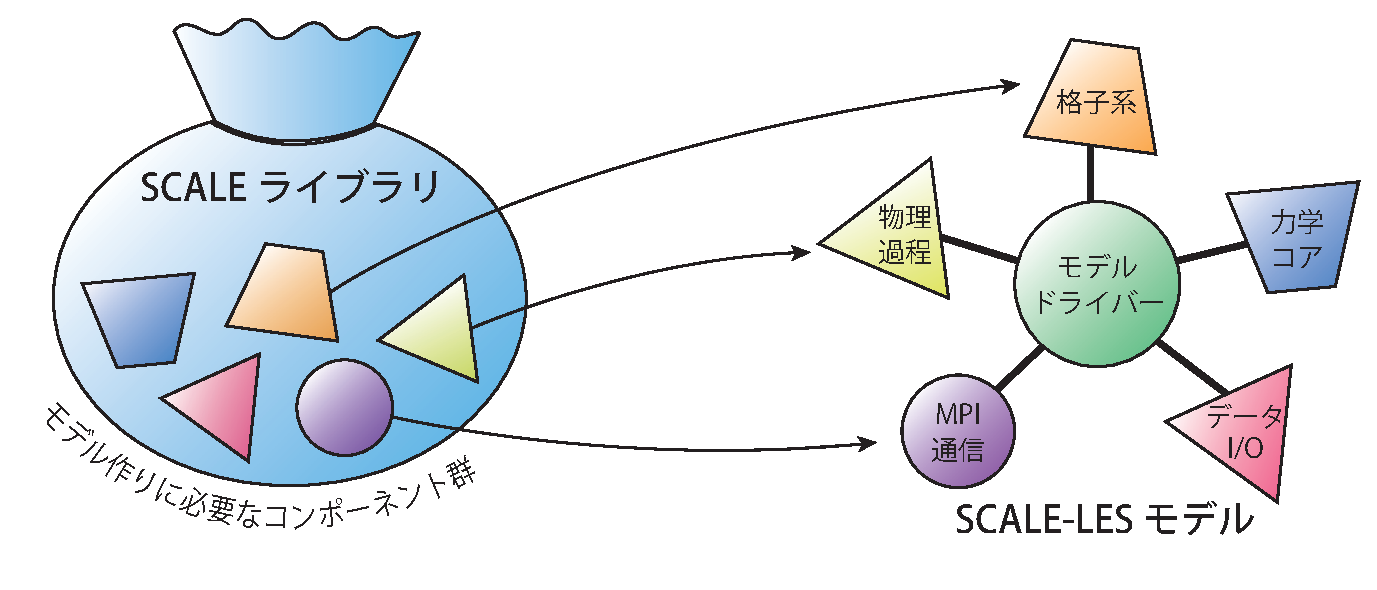
\includegraphics[width=0.9\hsize]{./figure/scale_and_scale-les.eps}\\
  \caption{SCALEライブラリとSCALE-LESモデルの関係}
  \label{fig:scale-les}
\end{center}
\end{figure}


\section{表記上の注意}

本書中のシェルコマンド等はbash を想定して記述する。異なる環境下では適宜読み替えて対応すること。
また、本書内では特に断りがない限り、下記の表記法に従うものとする。


コマンドラインのシンボル(\verb|$, #|)は、コマンドの実行を示す。
下記の表記の違いは、プログラムを実行する権限の違いを示している。

\begin{verbatim}
 #        <- root権限で実行するコマンド
 $        <- ユーザ権限で実行するコマンド
\end{verbatim}
権限の一時的な切り替えにはsuコマンドを用いる。
\verb|{User_Name}|は実際のユーザ名に読み替えること。
\begin{verbatim}
 $ su {User_Name}   <- {User_Name}のユーザー名でログイン
 $ exit             <- {User_Name}のユーザー名でログインを修了
 $ su -             <- root権限に変更
 #
\end{verbatim}

コマンドオプションにハイフンを用いると、そのユーザでのログインを行う。
用いない場合、権限のみの変更となる。またユーザ名を省略するとrootでのログインを試す。
ユーザの一時切り替えを終わるには、exitコマンドを用いる。
%各プログラムをインストールするための圧縮ファイルは、/tmpにダウンロードされていると仮定する。
%他のディレクトリにダウンロードしてある場合は、mvコマンド等を用いて/tmpに移動しておくことを勧める。
文章表記のうち、ダブルスラッシュ(//)で始まる行は解説のためのもので、実際に記述する必要はない。

下記のように四角い囲みで区切られた部分は、コマンドラインのメッセージ部分であることを意味する。\\
{\small {\gt
\fbox{
\begin{tabularx}{100mm}{l}
 -- -- -- -- コマンドラインのメッセージ\\
 -- -- -- -- -- -- -- -- コマンドラインのメッセージ\\
 -- -- -- -- -- -- -- -- -- -- -- -- コマンドラインのメッセージ\\
\end{tabularx}
}}}\\

また、下記のように丸い囲みで区切られた部分は、エディタでファイルを編集する記述内容を表す、
もしくはファイル内の記述を参照している部分である。\\
{\small {\gt
\ovalbox{
\begin{tabularx}{100mm}{l}
 -- -- -- -- ファイル中の記述\\
 -- -- -- -- -- -- -- -- ファイル中の記述\\
 -- -- -- -- -- -- -- -- -- -- -- -- ファイル中の記述\\
\end{tabularx}
}}}\\


\begin{verbatim}
 $ vi
\end{verbatim}

上記のコマンドは、vi(汎用テキストエディタ)プログラムを実行する。
他に、gedit、emacsなどのテキストエディタがある。
マニュアルではviコマンドの実行指示があるが、各自の使いやすいエディタへ適宜読み替えること。
